\section{Cơ sở toán học và cài đặt mô hình}
\label{sec:mo_hinh}

Chương này mô tả SVM và hồi quy logistic, từ hàm mục tiêu đến cách chọn cấu hình cho thực nghiệm. Ký hiệu $\mathbf{x}_i \in \mathbb{R}^d$ chỉ vectơ đầu vào của ảnh thứ $i$, với $d = 26.244$ cho HOG và $d = 256$ sau PCA. Ký hiệu $y_i$ là nhãn của ảnh, $n$ là số ảnh trong tập train và $K = 6$ là số lớp.

\subsection{Máy vectơ hỗ trợ (SVM)}
\label{sec:svm}

\subsubsection{Nguyên lý phân loại}

Trong bài toán hai lớp, SVM~\cite{cortes1995svm} tìm một siêu phẳng quyết định có lề (margin) rộng. Khi hai lớp phân tách tuyến tính, lề được xác định bởi các điểm gần siêu phẳng nhất. Với dữ liệu có các lớp chồng lấn, SVM cân bằng giữa độ rộng của lề và mức phạt khi mẫu huấn luyện vi phạm lề.

Trong dạng đối ngẫu, các mẫu có hệ số khác 0 được gọi là vectơ hỗ trợ (support vectors). Các vectơ này tham gia trực tiếp vào hàm quyết định, như trình bày ở phần SVM dùng hàm nhân.

SVM tuyến tính dùng ranh giới tuyến tính trong không gian HOG. SVM RBF áp dụng hàm nhân trên 256 thành phần PCA và có thể biểu diễn ranh giới phi tuyến trong không gian đầu vào này.

Vectơ HOG có hàng chục nghìn chiều nên không thể vẽ trực tiếp ranh giới quyết định của mô hình. Hình~\ref{fig:svm_boundary} vì vậy minh họa khác biệt giữa hai loại ranh giới trên một bộ dữ liệu hai lớp, hai chiều do nhóm tự sinh. Trên dữ liệu này, ranh giới thẳng của SVM tuyến tính cắt ngang cả hai lớp, còn ranh giới của SVM RBF uốn theo hình dạng của dữ liệu.

\begin{figure}[H]
  \centering
  \begin{subfigure}{0.62\textwidth}
    \centering
    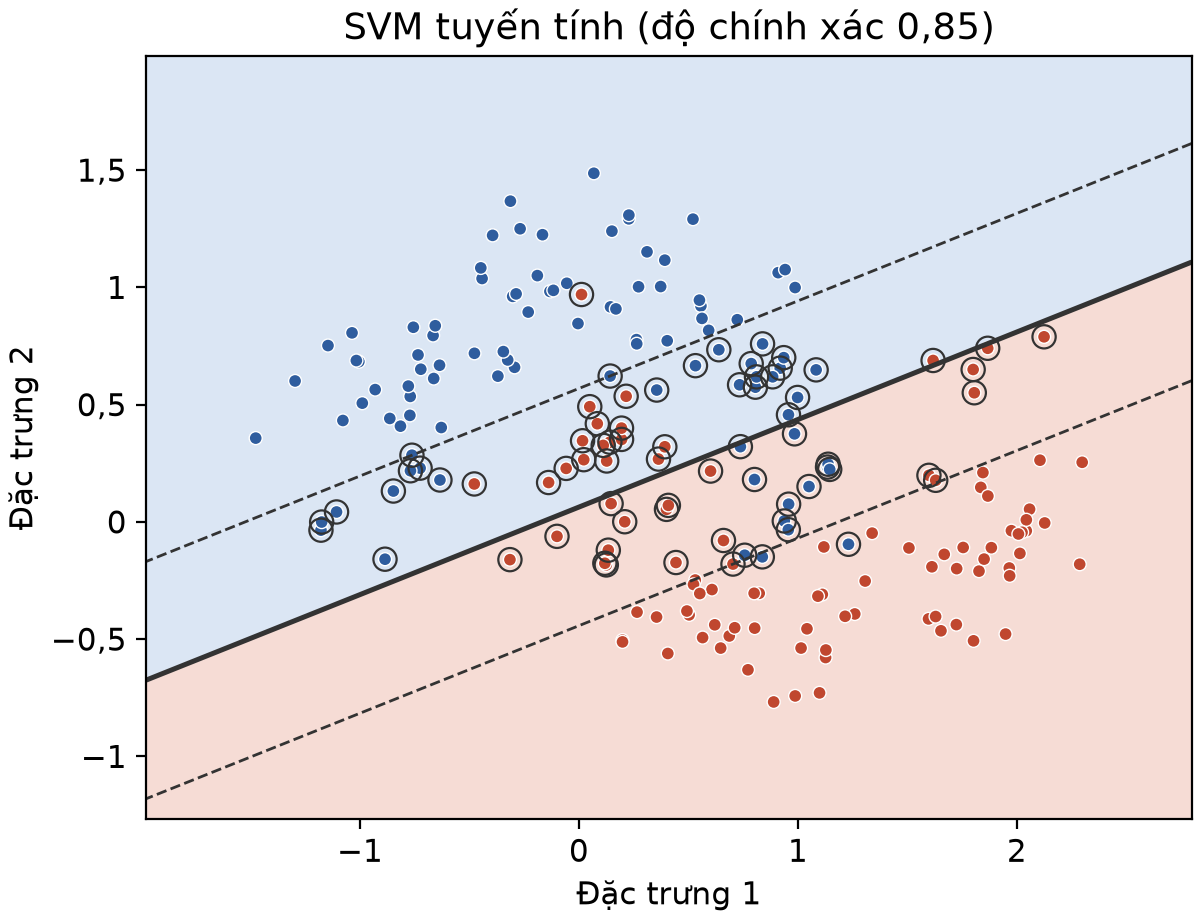
\includegraphics[width=\linewidth]{svm_boundary_linear.png}
    \caption{SVM tuyến tính}
    \label{fig:svm_boundary_linear}
  \end{subfigure}

  \vspace{0.4em}
  \begin{subfigure}{0.62\textwidth}
    \centering
    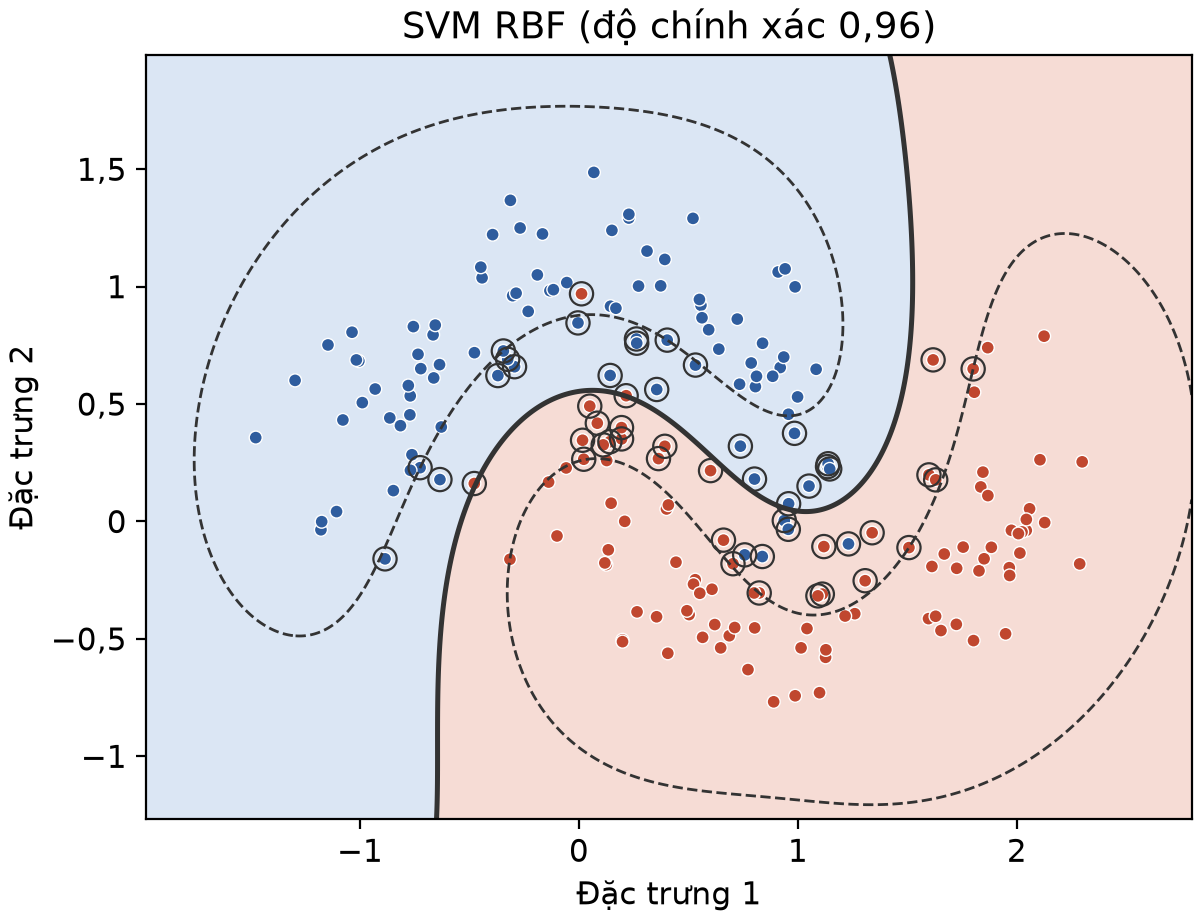
\includegraphics[width=\linewidth]{svm_boundary_rbf.png}
    \caption{SVM RBF}
    \label{fig:svm_boundary_rbf}
  \end{subfigure}
  \caption[Ranh giới quyết định của SVM tuyến tính và SVM RBF trên dữ liệu minh họa]{Ranh giới quyết định của SVM tuyến tính và SVM RBF trên dữ liệu minh họa hai chiều gồm hai lớp (200 điểm, $C = 1$). Màu của mỗi điểm là nhãn thật của điểm đó; màu nền là lớp mà mô hình dự đoán tại từng vị trí, nên điểm có màu khác với màu nền là điểm bị phân loại sai. Nét liền là ranh giới quyết định, nét đứt là lề, các điểm được khoanh tròn là vectơ hỗ trợ. Độ chính xác được tính trên chính dữ liệu minh họa.}
  \label{fig:svm_boundary}
\end{figure}

\subsubsection{Cơ sở toán học}

\paragraph{SVM tuyến tính cho hai lớp.} Với nhãn $y_i \in \{-1, +1\}$, SVM dự đoán bằng dấu của hàm
\[
  f(\mathbf{x}) = \mathbf{w}^\top \mathbf{x} + b .
\]
Khoảng cách giữa hai siêu phẳng lề $f(\mathbf{x}) = \pm 1$ bằng $2 / \lVert \mathbf{w} \rVert$. Vì vậy, mở rộng lề tương ứng với giảm chuẩn của $\mathbf{w}$. Dạng cơ bản của hàm mục tiêu tuyến tính với mất mát hinge bình phương (\emph{squared hinge}) và trọng số lớp đồng nhất là
\begin{equation}
  \min_{\mathbf{w},\, b} \;\; \frac{1}{2} \lVert \mathbf{w} \rVert^2
  \;+\; C \sum_{i=1}^{n} \max\!\bigl(0,\; 1 - y_i(\mathbf{w}^\top \mathbf{x}_i + b)\bigr)^2 ,
  \label{eq:linsvm}
\end{equation}
trong đó:
\begin{itemize}
  \item Số hạng $\frac{1}{2}\lVert \mathbf{w} \rVert^2$ khuyến khích lề rộng.
  \item Số hạng mất mát $\max(0, 1 - y_i f(\mathbf{x}_i))^2$ bằng 0 khi $y_i f(\mathbf{x}_i) \geq 1$. Giá trị này tăng theo bình phương của mức vi phạm lề.
  \item $C > 0$ điều chỉnh mức phạt đối với vi phạm lề. Giảm $C$ làm tăng mức điều chuẩn tương đối so với mất mát trên tập train.
\end{itemize}

\paragraph{Mở rộng cho nhiều lớp.} Nhóm dùng \texttt{LinearSVC} với chiến lược một lớp so với các lớp còn lại (one-vs-rest). Mỗi bộ phân loại tách một lớp khỏi năm lớp còn lại. Mô hình gán ảnh cho lớp có điểm quyết định $f_k(\mathbf{x})$ cao nhất.

\paragraph{Trọng số lớp.} Nhóm dùng chế độ trọng số cân bằng để tăng mức phạt cho các mẫu thuộc lớp có ít ảnh. Trọng số của lớp $k$ là
\begin{equation}
  s_k = \frac{n}{K \cdot n_k},
  \label{eq:classweight}
\end{equation}
trong đó $n_k$ là số ảnh trong tập train thuộc lớp $k$. Với dữ liệu của đồ án, $s_{\texttt{tarjeta}} = 6361 / (6 \cdot 297) \approx 3{,}57$ và $s_{\texttt{pistol}} = 6361 / (6 \cdot 2649) \approx 0{,}40$. Trọng số của lớp thẻ ngân hàng lớn gần gấp 9 lần trọng số của lớp súng ngắn.

\paragraph{SVM dùng hàm nhân.} Với hàm mất mát hinge và trọng số lớp đồng nhất, bài toán SVM có dạng đối ngẫu (dual) sau
\begin{equation}
  \max_{\bm{\alpha}} \; \sum_{i=1}^{n} \alpha_i - \frac{1}{2} \sum_{i=1}^{n} \sum_{j=1}^{n} \alpha_i \alpha_j y_i y_j \, K(\mathbf{x}_i, \mathbf{x}_j)
  \quad \text{với} \quad 0 \le \alpha_i \le C, \;\; \sum_{i=1}^{n} \alpha_i y_i = 0 ,
\end{equation}
và hàm quyết định trở thành
\begin{equation}
  f(\mathbf{x}) = \sum_{i=1}^{n} \alpha_i y_i \, K(\mathbf{x}_i, \mathbf{x}) + b .
\end{equation}
Các mẫu có $\alpha_i > 0$ là vectơ hỗ trợ. Vì vậy, chỉ các mẫu này đóng góp vào tổng trong hàm quyết định. Hàm nhân $K(\mathbf{x}_i, \mathbf{x}_j)$ xác định độ tương đồng trong không gian đặc trưng của mô hình. Hàm nhân tuyến tính có dạng $K(\mathbf{x}_i, \mathbf{x}_j) = \mathbf{x}_i^\top \mathbf{x}_j$. Hàm nhân RBF có dạng
\begin{equation}
  K(\mathbf{x}, \mathbf{x}') = \exp\!\bigl(-\gamma \lVert \mathbf{x} - \mathbf{x}' \rVert^2\bigr), \qquad \gamma > 0 .
  \label{eq:rbf}
\end{equation}
Hàm nhân RBF bằng 1 khi hai vectơ đầu vào bằng nhau và giảm khi khoảng cách giữa chúng tăng. Trong hàm quyết định, đóng góp của mỗi vectơ hỗ trợ phụ thuộc vào hệ số, nhãn lớp và khoảng cách đến vectơ cần phân loại.

Tham số $\gamma$ điều chỉnh tốc độ giảm của hàm nhân theo khoảng cách. Với cùng một khoảng cách, $\gamma$ càng lớn thì độ tương đồng càng thấp. Khi $\gamma$ nhỏ, các cặp vectơ có thể nhận giá trị hàm nhân gần nhau. Nhóm khảo sát chế độ \texttt{"scale"} của scikit-learn, trong đó
\begin{equation}
  \gamma = \frac{1}{d \cdot \operatorname{Var}(\mathbf{X})},
  \label{eq:gammascale}
\end{equation}
với $\operatorname{Var}(\mathbf{X})$ là phương sai tính trên toàn bộ phần tử của ma trận đầu vào dùng khi huấn luyện. Chế độ này đặt $\gamma$ theo số chiều và thang đo của dữ liệu. Mục~\ref{sec:svm_tuning} so sánh kết quả với hai giá trị $\gamma$ cố định.

\paragraph{Mở rộng SVM RBF cho nhiều lớp.} Nhóm dùng \texttt{SVC} với chiến lược phân loại từng cặp lớp (one-vs-one). Với sáu lớp, mô hình huấn luyện $K(K-1)/2 = 15$ bộ phân loại nhị phân và dự đoán dựa trên kết quả biểu quyết của các bộ phân loại này.

\subsubsection{Các siêu tham số quan trọng}

Bảng~\ref{tab:svm_hparams} trình bày các giá trị được khảo sát hoặc cố định cho hai biến thể SVM. Nhóm thử các giá trị $C$ và $\gamma$ ở nhiều bậc độ lớn.

\begin{table}[H]
\centering
\caption{Siêu tham số của hai biến thể SVM}
\label{tab:svm_hparams}
\small
\begin{tabularx}{\textwidth}{@{}l X X@{}}
\toprule
\textbf{Siêu tham số} & \textbf{SVM tuyến tính} & \textbf{SVM RBF} \\
\midrule
Đầu vào            & 26.244 đặc trưng HOG đã chuẩn hóa & 256 thành phần PCA \\
$C$ (tìm kiếm)     & $\{0{,}001;\ 0{,}01;\ 0{,}1;\ 1;\ 10;\ 100\}$ & $\{1;\ 10;\ 50\}$ \\
$\gamma$ (tìm kiếm) & -- & $\{\texttt{"scale"};\ 0{,}01;\ 0{,}001\}$ \\
Hàm mất mát        & Hinge bình phương & Hinge (dạng đối ngẫu) \\
Chiến lược đa lớp & Một lớp so với các lớp còn lại (6 bộ) & Từng cặp lớp (15 bộ) \\
Trọng số lớp       & Cân bằng & Cân bằng \\
Số vòng lặp tối đa & 5.000 & Không giới hạn \\
\bottomrule
\end{tabularx}
\end{table}

Khi huấn luyện SVM tuyến tính, nhóm ước lượng vectơ trọng số $\mathbf{w}_k$ và hệ số chặn $b_k$ cho từng bộ phân loại. Với SVM RBF, quá trình huấn luyện xác định các vectơ hỗ trợ cùng hệ số của chúng.

\subsubsection{Cài đặt}

Nhóm dùng scikit-learn để huấn luyện hai biến thể SVM trên từng nhánh tiền xử lý.

\textbf{Bước 1. Tinh chỉnh $C$ cho SVM tuyến tính.} Với mỗi giá trị $C$, nhóm huấn luyện mô hình trên tập train và tính macro-F1 trên tập validation. Nhóm giữ giá trị $C$ có macro-F1 cao nhất.

\begin{lstlisting}[caption={Tinh chỉnh $C$ cho SVM tuyến tính (rút gọn)},label={lst:tune_linear}]
scaler = StandardScaler(with_mean=False)
X_tr = scaler.fit_transform(X_train)        # fit on training set only
X_va = scaler.transform(X_val)

best_c, best_f1 = None, -1.0
for c in [0.001, 0.01, 0.1, 1.0, 10.0, 100.0]:
    clf = LinearSVC(C=c, class_weight="balanced",
                    max_iter=5000, dual="auto", random_state=42)
    clf.fit(X_tr, y_train)
    f1 = f1_score(y_val, clf.predict(X_va), average="macro")
    if f1 > best_f1:
        best_c, best_f1 = c, f1
\end{lstlisting}

\textbf{Bước 2. Huấn luyện mô hình tuyến tính cuối cùng.} Nhóm ghép bộ chuẩn hóa và SVM tuyến tính thành một quy trình xử lý (\emph{pipeline}). Quy trình dùng giá trị $C$ đã chọn, được huấn luyện lại trên tập train và được đánh giá trên hai tập còn lại. Khi dự đoán trên ảnh mới, vectơ HOG đi qua cùng bộ chuẩn hóa trước khi vào bộ phân loại.

\textbf{Bước 3. Giảm chiều bằng PCA.} Nhóm ước lượng bộ chuẩn hóa và PCA từ tập train. Sau đó, nhóm dùng cùng phép biến đổi để chiếu dữ liệu của ba tập vào không gian 256 chiều.

\begin{lstlisting}[caption={Giảm chiều trước SVM RBF (rút gọn)},label={lst:pca}]
pca_scaler = StandardScaler(with_mean=False)
X_tr_sc = pca_scaler.fit_transform(X_train)
pca = PCA(n_components=256, svd_solver="randomized", random_state=42)
X_tr_pca = pca.fit_transform(X_tr_sc)                 # fit on training set only
X_va_pca = pca.transform(pca_scaler.transform(X_val))
X_te_pca = pca.transform(pca_scaler.transform(X_test))
\end{lstlisting}

\textbf{Bước 4. Tinh chỉnh và huấn luyện SVM RBF.} Nhóm huấn luyện chín cấu hình từ ba giá trị $C$ và ba giá trị $\gamma$, rồi chọn cấu hình có macro-F1 cao nhất trên tập validation. Quy trình lưu để dự đoán gồm bộ chuẩn hóa, PCA và bộ phân loại SVM RBF. Đầu vào của quy trình là vectơ HOG.

\begin{lstlisting}[caption={Tinh chỉnh và lưu SVM RBF (rút gọn)},label={lst:rbf}]
results = []
for c in [1.0, 10.0, 50.0]:
    for g in ["scale", 0.01, 0.001]:
        clf = SVC(C=c, gamma=g, kernel="rbf", class_weight="balanced")
        clf.fit(X_tr_pca, y_train)
        f1 = f1_score(y_val, clf.predict(X_va_pca), average="macro")
        results.append((f1, c, g))
_, best_c, best_g = max(results)

rbf = SVC(C=best_c, gamma=best_g, kernel="rbf", class_weight="balanced")
rbf.fit(X_tr_pca, y_train)
model = Pipeline([("scaler", pca_scaler), ("pca", pca), ("clf", rbf)])
joblib.dump(model, MODEL_PATH)
\end{lstlisting}

\subsection{Hồi quy logistic (Logistic Regression)}
\label{sec:lr}

\subsubsection{Nguyên lý phân loại}

Hồi quy logistic tính điểm số tuyến tính cho từng lớp, sau đó dùng hàm softmax để ước lượng xác suất thuộc từng lớp. Mô hình gán ảnh cho lớp có xác suất ước lượng cao nhất.

Nhóm huấn luyện mô hình bằng hàm mất mát entropy chéo có điều chuẩn. Để khảo sát ảnh hưởng của việc giảm số đặc trưng, nhóm so sánh mô hình dùng toàn bộ vectơ HOG với các biến thể dùng bộ lọc ANOVA, trong đó một biến thể kết hợp thêm điều chuẩn L1.

\subsubsection{Cơ sở toán học}

\paragraph{Mô hình.} Với mỗi lớp $k$, mô hình tính một điểm số tuyến tính
\[
  z_k = \mathbf{w}_k^\top \mathbf{x} + b_k , \qquad k = 1, \dots, K ,
\]
rồi chuyển $K$ điểm số thành $K$ xác suất có tổng bằng 1 bằng hàm softmax:
\begin{equation}
  \hat{p}_k(\mathbf{x}) = P(y = k \mid \mathbf{x}) = \frac{\exp(z_k)}{\sum_{j=1}^{K} \exp(z_j)} .
  \label{eq:softmax}
\end{equation}
Khi $K = 2$, xác suất của một lớp có thể viết dưới dạng sigmoid $\sigma(z) = 1/(1 + e^{-z})$, với $z$ là chênh lệch giữa hai điểm số.

\paragraph{Hàm mất mát.} Khi huấn luyện, nhóm dùng tổng mất mát entropy chéo (cross-entropy) có trọng số lớp
\begin{equation}
  \mathcal{L}(\mathbf{W}, \mathbf{b}) = - \sum_{i=1}^{n} s_{y_i} \log \hat{p}_{y_i}(\mathbf{x}_i) ,
  \label{eq:ce}
\end{equation}
trong đó $s_{y_i}$ là trọng số lớp theo công thức~\eqref{eq:classweight}. Nếu mô hình gán xác suất 0,01 cho nhãn đúng, mẫu đó đóng góp khoảng $4{,}6 s_{y_i}$ vào hàm mất mát. Khi đánh giá, nhóm báo cáo log-loss dưới dạng trung bình mất mát trên mỗi ảnh, với trọng số như nhau cho mọi ảnh.

\paragraph{Điều chuẩn.} Hàm mục tiêu bổ sung một số hạng phạt độ lớn của trọng số. Hai dạng được dùng trong đồ án là
\begin{align}
  \text{Điều chuẩn L2:} \quad & \min_{\mathbf{W}, \mathbf{b}} \; \frac{1}{2} \sum_{k=1}^{K} \lVert \mathbf{w}_k \rVert_2^2 + C \cdot \mathcal{L}(\mathbf{W}, \mathbf{b}) , \label{eq:l2}\\
  \text{Điều chuẩn L1:} \quad & \min_{\mathbf{W}, \mathbf{b}} \; \sum_{k=1}^{K} \lVert \mathbf{w}_k \rVert_1 + C \cdot \mathcal{L}(\mathbf{W}, \mathbf{b}) . \label{eq:l1}
\end{align}
Khi $C$ giảm, số hạng điều chuẩn có ảnh hưởng lớn hơn so với mất mát huấn luyện. Điều chuẩn L2 khuyến khích hệ số có độ lớn nhỏ. Điều chuẩn L1 có thể đưa một số hệ số về đúng 0. Trong mô hình đa lớp, một đặc trưng chỉ ngừng đóng góp vào mọi điểm số nếu hệ số của nó bằng 0 ở tất cả các lớp.

\paragraph{Thuật toán tối ưu.} Với điều chuẩn L2, nhóm dùng L-BFGS, một phương pháp tựa Newton (quasi-Newton) xấp xỉ thông tin về độ cong từ các lần cập nhật trước. Với điều chuẩn L1, nhóm dùng SAGA, thuật toán hỗ trợ số hạng điều chuẩn không khả vi tại 0.

\paragraph{Lọc đặc trưng bằng ANOVA.} Nhóm tính thống kê $F$ cho từng đặc trưng và giữ $k$ đặc trưng có điểm cao nhất. Với đặc trưng $j$, thống kê này có dạng
\begin{equation}
  F_j = \frac{\text{bình phương trung bình giữa các lớp}}{\text{bình phương trung bình trong các lớp}} .
\end{equation}
$F_j$ lớn khi mức chênh lệch giữa các trung bình lớp lớn so với mức biến thiên trong từng lớp. Vì phép lọc chấm điểm từng đặc trưng riêng lẻ, nó có thể bỏ qua những đặc trưng chỉ hữu ích khi xét cùng các đặc trưng khác.

\paragraph{Lựa chọn đặc trưng bằng điều chuẩn L1.} Điều chuẩn L1 tác động đồng thời lên các hệ số trong khi huấn luyện. Trong thí nghiệm này, nhóm áp dụng L1 cho 8.000 đặc trưng đã qua bộ lọc ANOVA.

\subsubsection{Các siêu tham số quan trọng}

\begin{table}[H]
\centering
\caption{Cấu hình các biến thể hồi quy logistic}
\label{tab:lr_hparams}
\small
\begin{tabularx}{\textwidth}{@{}l X@{}}
\toprule
\textbf{Siêu tham số} & \textbf{Giá trị} \\
\midrule
Đầu vào & 26.244 đặc trưng HOG của nhánh \emph{padding}, đã chuẩn hóa \\
$C$ & Cố định bằng 1,0 cho mọi biến thể (không tinh chỉnh) \\
Điều chuẩn & L2 cho mô hình cơ sở và các biến thể lọc ANOVA. L1 cho biến thể kết hợp ANOVA với điều chuẩn L1. \\
Số đặc trưng giữ lại sau lọc ANOVA & $\{1.000;\ 3.000;\ 8.000\}$ \\
Thuật toán tối ưu & L-BFGS cho L2, tối đa 1.000 vòng lặp; SAGA cho L1, tối đa 300 vòng lặp, ngưỡng dừng $10^{-3}$ \\
Trọng số lớp & Cân bằng \\
\bottomrule
\end{tabularx}
\end{table}

Nhóm giữ $C = 1{,}0$ cho cả năm biến thể hồi quy logistic. Các kết quả so sánh vì vậy chỉ áp dụng cho những cấu hình tại giá trị này. Biến thể L1 còn dùng thuật toán tối ưu và điều kiện dừng khác với các biến thể L2.

\subsubsection{Cài đặt}

Nhóm huấn luyện hồi quy logistic trên CPU của Google Colab, dùng nhánh \emph{padding} và cùng cách chia tập với SVM.

\textbf{Mô hình cơ sở.} Nhóm dùng toàn bộ 26.244 đặc trưng. Quy trình xử lý ước lượng bộ chuẩn hóa và mô hình trên tập train.

\begin{lstlisting}[caption={Mô hình hồi quy logistic cơ sở},label={lst:lr_base}]
m_base = make_pipeline(
    StandardScaler(),
    LogisticRegression(C=1.0, max_iter=1000, class_weight="balanced"))
m_base.fit(Xtr, ytr)
\end{lstlisting}

\textbf{Lọc đặc trưng bằng ANOVA.} Với mỗi giá trị $k$, nhóm tính thống kê $F$ trên tập train và giữ $k$ đặc trưng có điểm cao nhất. Sau đó, nhóm huấn luyện hồi quy logistic trên các đặc trưng đã chọn.

\begin{lstlisting}[caption={Lựa chọn đặc trưng bằng thống kê ANOVA},label={lst:lr_kbest}]
scaler = StandardScaler().fit(Xtr)
S_tr, S_va = scaler.transform(Xtr), scaler.transform(Xva)

for k in [1000, 3000, 8000]:
    sel = SelectKBest(f_classif, k=k).fit(S_tr, ytr)
    m = LogisticRegression(C=1.0, class_weight="balanced", max_iter=1000)
    m.fit(sel.transform(S_tr), ytr)
\end{lstlisting}

\textbf{Kết hợp ANOVA và điều chuẩn L1.} Nhóm giữ 8.000 đặc trưng theo thống kê ANOVA rồi dùng điều chuẩn L1 trong hồi quy logistic. Sau khi huấn luyện, nhóm đếm số hệ số khác 0 trên cả sáu lớp.

\begin{lstlisting}[caption={Hồi quy logistic với điều chuẩn L1},label={lst:lr_l1}]
A8 = sel8k.transform(S_tr)            # 8000 features kept by ANOVA
m_l1 = LogisticRegression(penalty="l1", solver="saga", C=1.0,
                          class_weight="balanced", max_iter=300, tol=1e-3)
m_l1.fit(A8, ytr)
nonzero = (m_l1.coef_ != 0).sum()     # number of non-zero weights
\end{lstlisting}

\textbf{Chọn biến thể cuối cùng.} Nhóm so sánh năm biến thể trên tập validation và đánh giá biến thể có macro-F1 cao nhất trên tập test.
